\begin{frame}
\frametitle{Поток исполнения}
\begin{itemize}
  \item Поток исполнения (aka поток) - память содержащая команды и некоторый
  контекст, определяющий состояние потока исполнения
  \begin{itemize}
    \item набор команд и то что нужно для их исполнения.
  \end{itemize}
  \item Контекст потока - окружение в котором исполняются команды и состояние
  CPU:
  \begin{itemize}
    \item доступная память:
    \begin{itemize}
      \item таблица страниц определяет всю доступную память (если вы ее
      используете);
      \item память с командами и данными;
      \item стек;
    \end{itemize}
    \item регистры процессора.
  \end{itemize}
\end{itemize}
\end{frame}

\begin{frame}
\frametitle{Память потока}
\begin{itemize}
  \item Различные потоки исполнения \emph{могут} "разделять" общую память:
  \begin{itemize}
    \item использовать один и тот же набор команд;
    \item работать с одними и теми же данными;
    \item однако потоки могут быть и изолированы друг от друга, например, иметь
    свою таблицу страниц.
  \end{itemize}
  \item Стек у каждого потока свой:
  \begin{itemize}
    \item стек важная область памяти для исполнения команд потока;
    \item стек хранит локальные переменные функций;
    \item на стек, \emph{обычно}, сохраняются адреса возврата при вызове
    функций.
  \end{itemize}
\end{itemize}
\end{frame}

\begin{frame}
\frametitle{Состояние CPU}
\begin{itemize}
  \item Состояние CPU включает:
  \begin{itemize}
    \item регистры общего назначения:
    \begin{itemize}
      \item например, для x86-64 это регистры RAX, RBX, RCX, RDX, RDI, RSI,
      RBP, RSP, R9-R15;
    \end{itemize}
    \item флаговый регистр (или регистры):
    \begin{itemize}
      \item регистры флагов используются для организации условных переходов или
      условного исполнения;
      \item например, для x86-64 это регистр RFLAGS;
    \end{itemize}
    \item прочие регистры, участвующие в вычислениях:
    \begin{itemize}
      \item например, xmm/avx/прочие регистры x86 используемые для
      floating-point арифметики и SIMD инструкций, которые не будут
      интересовать нас в домашних заданиях.
    \end{itemize}
  \end{itemize}
\end{itemize}
\end{frame}

\begin{frame}
\frametitle{Многопоточность}
\begin{itemize}
  \item Одновременно могут исполняться сразу несколько потоков:
  \begin{itemize}
    \item если на одном кристалле находится сразу несколько полноценных или не
    очень (aka Hyper Threading) вычислительных ядер;
    \item если у вас просто несколько CPU в системе.
  \end{itemize}
  \item Потоки могут исполняться \emph{почти} одновременно:
  \begin{itemize}
    \item одновременность в контексте многопточности - плохое слово (вообще
    понятие времени очень странное в данном контексте);
    \item в каждый момент времени на конкретном CPU исполняется только один
    поток, но между потоками можно быстро переключаться создавая иллюзию
    одновременной работы.
  \end{itemize}
\end{itemize}
\end{frame}

\begin{frame}
\frametitle{Кооперативная и вытесняющая многопточность}
\begin{itemize}
  \item Кооперативная многопоточность
  \begin{itemize}
    \item поток работает на CPU до тех пор, пока он сам не решит "отдать" CPU
    кому-нибудь другому;
    \item часто в некоторых контекстах такие потоки называют корутинами;
    \item считается, что программировать используя кооперативную многопточность
    проще (впрочем, это очень-очень-очень спорное утверждение).
  \end{itemize}
  \item Вытесняющая многопоточность
  \begin{itemize}
    \item поток может быть смещен (вытеснен) c CPU в любой момент без
    предупреждения;
    \item например, ОС может смещать поток с CPU, если он отработал достаточно
    долго;
    \item поток все еще может сам отдать CPU.
  \end{itemize}
\end{itemize}
\end{frame}

\begin{frame}
\frametitle{Переключенние потоков}
\begin{itemize}
  \item Для переключения потоков, очевидно, нужно подменить контекст одного
  потока, контекстом другого потока и передать управление коду другого потока
  \begin{itemize}
    \item чтобы уметь переключиться назад на старый поток необходимо сохранить
    его контекст, чтобы его можно было восстановить;
    \item переключением с одного потока на другой поток занимается какой-то
    код, этот код тоже использует регистры и какую-то память;
    \item соответственно, это код не должен в процессе сохранения состояния
    испортить само состояние;
    \item соответственно, код переключающий потоки должен быть доступен в каждом
    потоке - все потоки должны иметь какую-то общую память.
  \end{itemize}
\end{itemize}
\end{frame}

\begin{frame}[fragile]
\frametitle{Пример переключения для x86}
\begin{columns}
  \begin{column}{0.4\linewidth}
    \begin{lstlisting}
    .text
switch_threads:
    pushq %rbx
    pushq %rbp
    pushq %r12
    pushq %r13
    pushq %r14
    pushq %r15
    pushfq

    movq %rsp, (%rdi)
    movq %rsi, %rsp

    popfq
    popq %r15
    popq %r14
    popq %r13
    popq %r12
    popq %rbp
    popq %rbx

    ret
    \end{lstlisting}
  \end{column}
  \begin{column}{0.6\linewidth}
    \begin{lstlisting}
void switch_thread(void **prev,void *next);
    \end{lstlisting}
    \begin{itemize}
      \item сохраняет состояние старого потока на стек:
      \begin{itemize}
        \item через \emph{prev} (регистр rdi) возвращается указатель на
        сохраненное состояние;
        \item \emph{next} (регистр rsi) - указатель на сохраненное состояние
        нового потока;
      \end{itemize}
    \end{itemize}
  \end{column}
\end{columns}
\end{frame}

\begin{frame}
\frametitle{Пример переключения для x86}
\begin{center}
  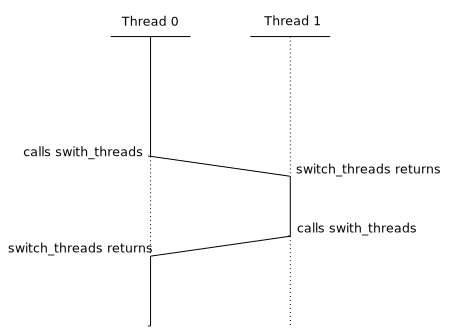
\includegraphics[width=0.5\linewidth]{switch_threads.png}
\end{center}
\begin{itemize}
  \item Функция \emph{switch\_threads} изменяет внутри себя регистр \emph{rsp}
  \begin{itemize}
    \item т. е. входим мы в функию пользуясь стеком \emph{Thread 0}, а выходим
    уже используя стек \emph{Thread 1};
    \item следовательно \emph{ret} берет адрес возврата со стека
    \emph{Thread 1}, т. е. \emph{ret} передает управление коду \emph{Thread 1}.
  \end{itemize}
\end{itemize}
\end{frame}

\begin{frame}
\frametitle{Пример переключения для x86}
\begin{itemize}
  \item \emph{switch\_threads} восстанавливает состояние сохраненное другим
  вызовом \emph{switch\_threads}
  \begin{itemize}
    \item как переключиться на поток в первый раз?
    \item при создании нового потока необходимо аллоцировать память под стек;
    \item мы можем искуственно "положить" на стек потока нужное "состояние";
  \end{itemize}
  \item под состоянием понимаются не только регистры сохраняемые командами
  \emph{pushq} и \emph{pushfq}, но и адрес возврата используемый инструкцией
  \emph{ret}
  \begin{itemize}
    \item по завершению \emph{switch\_threads} управление передается инструкцией
    \emph{ret} по адресу возврата сохраненному на стеке;
    \item т. е. адрес возврата - точка входа в наш поток (другими словами,
    main).
  \end{itemize}
\end{itemize}
\end{frame}

\begin{frame}
\frametitle{Организация вытесняющей многопоточности}
\begin{itemize}
  \item Имея \emph{switch\_threads} легко организовать кооперативную
  многопоточность
  \begin{itemize}
    \item достаточно узнать, где хранится состояние следующего потока.
  \end{itemize}
  \item Как организовать "насильное" вытеснение потока?
  \begin{itemize}
    \item необходимо "прерывать" исполняющийся на CPU код, и вызвать код,
    который выполнит переключение;
    \item для этого можно использовать прерывания (например, прерывание от
    таймера):
    \begin{itemize}
      \item обработчик прерывания прерывает исполняемый код, но в остальном
      выполняется в контексте прерваного кода;
      \item мы можем просто вызвать \emph{switch\_threads} из обработчика
      прерывания;
      \item не забудьте про EOI перед переключением.
    \end{itemize}
  \end{itemize}
\end{itemize}
\end{frame}

\begin{frame}
\frametitle{Организация вытесняющей многопоточности}
\begin{center}
  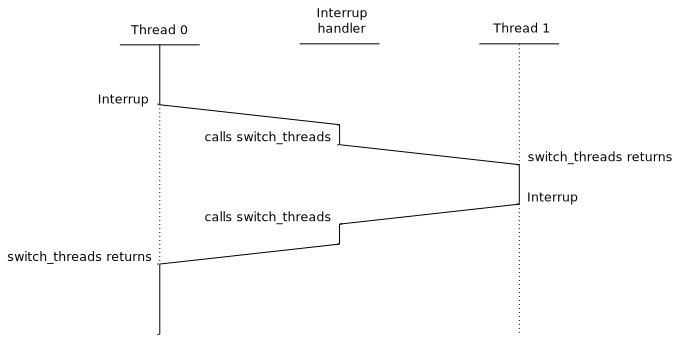
\includegraphics[width=0.8\linewidth]{switch_threads_preemptive.png}
\end{center}
\begin{itemize}
  \item CPU при вызове обработчика прерываний вытесняет исполняемый код с CPU;
  \item обработчик прерывания вызывает \emph{switch\_threads}.
\end{itemize}
\end{frame}
